\chapter{The System at a Glance}
\label{chap:overview}
% Traceability: ADR-001 ADR-002 ADR-003 ADR-004 ADR-005 ADR-006

The controller is a set of boards connected through a backplane. Each board has a clear role. The boards share power, safety signals, and timing, but they do not depend on one central processor for all their work.

A remote host operates the complete instrument. It communicates directly with every active board over Ethernet. Function boards perform detector-specific work. The main board coordinates the system. The backplane provides the common physical and electrical infrastructure.

Figure~\ref{fig:system-overview} shows this arrangement. It is a simple system view, not a wiring diagram. Later chapters explain each connection in more detail.

\begin{figure}[htbp]
  \centering
  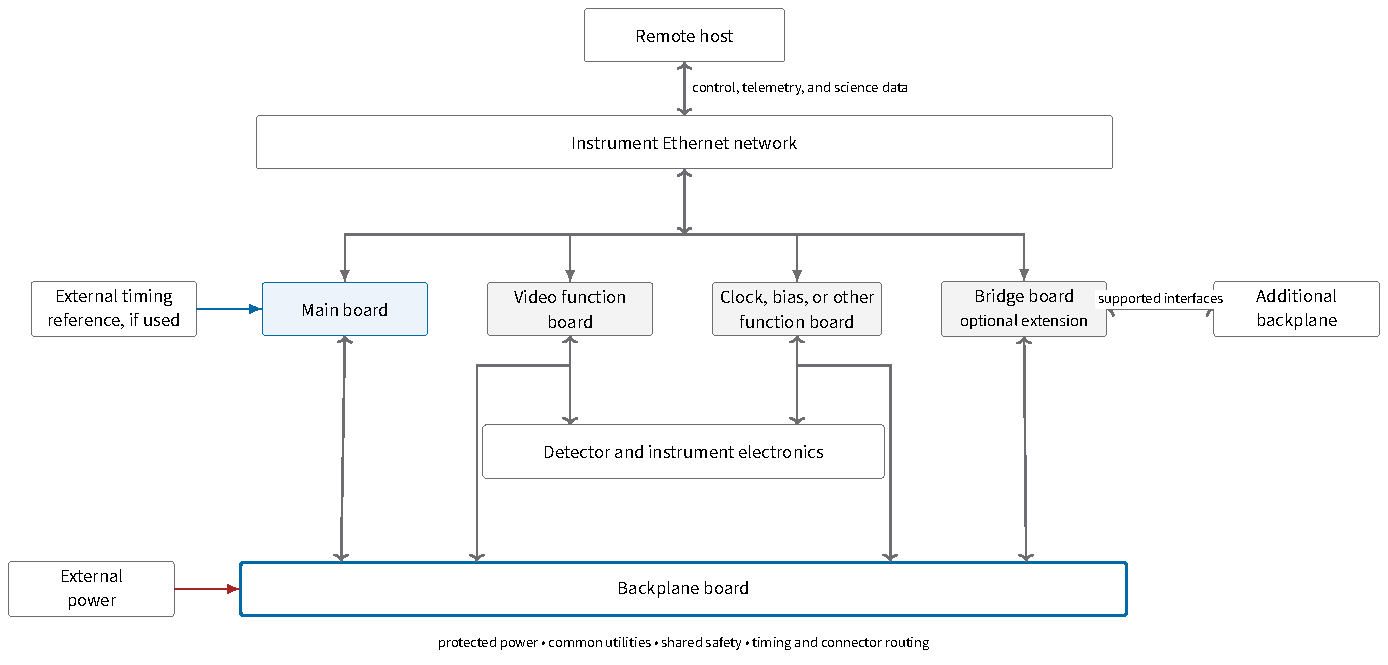
\includegraphics[width=\textwidth]{figures/generated/system_overview.tikz.pdf}
  \caption{High-level controller structure. Science data travels directly between the host and the function board that produces it; it does not pass through the main board.}
  \label{fig:system-overview}
\end{figure}

\section{Board Roles}

The architecture uses five board roles. A controller may contain several function boards and may use a bridge when it needs more than one backplane.

\begin{center}
\begin{tabularx}{\textwidth}{@{}>{\bfseries}p{0.22\textwidth}X@{}}
\toprule
Board role & Main purpose \\
\midrule
Main board & Coordinates system-wide enable, recovery, timing, and synchronization. It also observes shared health. It does not collect all science data or control the internal work of every function board. \\
Function board & Performs detector-specific work such as video acquisition, clock generation, or bias generation. Each active function board has its own control and network endpoint. \\
Backplane board & Holds the slots and distributes protected power, common utility rails, shared safety signals, timing, and connector routing. \\
Bridge board & Extends the supported shared interfaces to another backplane when the system must grow. \\
Passive terminator & Completes the safety continuity path in an unused slot. It has no active electronics. \\
\bottomrule
\end{tabularx}
\end{center}

The main board coordinates the controller, but it is not the controller's only intelligent element. Each active board manages its own local function, reports its status, and responds to the shared safety rules. This keeps the main board from becoming a processing or data bottleneck.

\section{The Four Main Connections}

Four types of connection make the separate boards operate as one controller.

\subsection{Power}

External power enters the backplane and passes through central input protection. The protected bulk supply then feeds every active board and the backplane utility converters. Common analog utility rails are available to boards that need them. Each board generates its ordinary digital supplies locally from the protected bulk supply.

\subsection{Safety and coordination}

The boards share a hardware fault path. Any participating board or supervised common rail can place the controller in a safe condition. The main board also provides the common arm and recovery signals. Detector-facing outputs remain off until both the system and the local board allow them to operate.

Software is used to identify and report the cause after the hardware has made the system safe. A lost host connection, failed processor, or missing acquisition clock must not prevent the required safety response.

\subsection{Timing}

The main board distributes the clock and synchronization events used for detector acquisition. Function boards use these signals when their work must align with other boards. Each active board also has an independent local clock for management, communication, and fault monitoring. Losing the acquisition clock therefore stops synchronized work without removing the board's ability to report the fault.

\subsection{Communication and science data}

Every active board has a direct Ethernet connection to the host. The host keeps the instrument inventory, maps each logical role to the correct board, sends configuration, and reads status.

Science data follows the same direct principle. A video board sends its data to the host instead of routing it through the main board or through a shared backplane data concentrator. This allows data capacity to grow as video boards and network capacity are added.

\section{A Normal Operating Cycle}

The complete controller follows a simple operating story:

\begin{enumerate}
  \item \textbf{Start safely.} Boards power up with detector-facing outputs disabled. They check local power, logic, timing, communication, and shared health.
  \item \textbf{Configure the instrument.} The host identifies the active boards and sends the settings and sequencer data needed for the current session.
  \item \textbf{Arm deliberately.} The host checks readiness and requests arming. Main checks its own conditions and raises \texttt{EN}. Each function board independently decides whether it can accept the arm request.
  \item \textbf{Acquire data.} The main board sends synchronized events. Function boards execute their local timing and data tasks. Video boards send science data directly to the host.
  \item \textbf{Disarm or go safe.} Stopping acquisition may leave the controller armed. Disarming drops \texttt{EN} and removes detector-facing permission. A trip removes permission through the interlock and requires explicit recovery.
  \item \textbf{Recover explicitly.} Restoring a missing clock, rail, or network link does not restart acquisition. The host requests recovery, the boards repeat their checks, and the system must be armed again.
\end{enumerate}

Chapter~\ref{chap:lifecycle} follows these actions through the operating states.

\medskip
\noindent\textit{Chapter sources:} ADR-001 through ADR-006 and the repository system concept guide. The ADRs remain authoritative for technical behavior.
